\documentclass{article}
\usepackage[utf8]{inputenc}
\usepackage{graphicx}
	\DeclareGraphicsExtensions{.png, .jpeg}
\usepackage{caption}
% \usepackage{subcaption}
\usepackage{csvsimple}
\usepackage[top=1in, bottom=1in, left=1in, right=1in]{geometry}

\title{PA04: Vector Reduce Revisited\\CS791v: Parallel Computing}
\author{Terence Henriod}
\date{\today}

\begin{document}

\clearpage
\maketitle
\thispagestyle{empty} % removes the page number from the title page

\begin{abstract}
In this assignment, we revisit vector reduction techniques on the GPU, this time attempting an array of techniques instead of just one. The first is vector reduction via kernel calls from the CPU; the second is reduction using a in itial kernel to pre-sum the elements followed by a final reduction kernel launch from within the original kernel; third is using the GPU to initially reduce the vector to an intermediate vector, and then complete the summation on the CPU; the final version is to use the \texttt{threadfence} instruction to have one block perform the final summation of the intermediate vector.
\end{abstract}

\newpage
\section{Introduction}
Vector reduction is a common, highly parallelizable task. It also provides ample flexibility to explore different GPU techniques in a simplified way. Even though reduction is typically summarized as simply ``summing all of the elements of a vector," the addition operation can be substituted to adapt reduction to a variety of tasks. Since elements can be operated on in any order, and only need to be operated only once, 

\section{Theory}
Here we discuss the methodologies of the various methods.

\subsection{Reduction Through Multiple Kernel Launches}
The most ``naive" way to reduce a vector. A kernel is used to task blocks with reducing the original vector into an intermediate vector that has as many elements as there were blocks in the kernel launch. In order to complete the reduction, the intermediate vector needs to be reduced once all of the blocks have completed their task. Since inter-block synchronization is difficult and costly to implement on hardware, the programmer can effect the inter-block synchronization by simply making a second kernel call that uses a single block to reduce the intermediate vector to a single element.

\subsection{Reduction Through Kernels That Launch Kernels}






\subsection{Reduction With a Kernel Launch and Final Reduction on the CPU}
While the GPU can provide large speedups through its massive parallelism, GPU kernels have high start-up and tear down costs, not to mention the need for memory transfers. Because of this, it can be beneficial to have smaller tasks be completed on the CPU. This way the CPU's quickness can be applied without large startup costs or memory transfers. In vector reduction, this takes the form of having the CPU perform the final reduce on the intermediate vector.

\subsection{Reduction With a Single Kernel and Inter-Block Synchronization}
As mentioned previously, inter-block synchronization is costly to implement, and so it is not done. Mostly. There is a special thread synchronization function known as \texttt{threadfence}. This instruction allows GPU code to make guarantees about the order of some operations. Using the \texttt{threadfence}, a vector can be reduced to an intermediate vector, then the fence can synchronize operations, and then the intermediate vector can be passed to a single block for final reduction. 

\newpage
\section{Results}
The performance results of the various vector reduction methods are displayed here.

\subsection{Information on the GPU device used}
\csvautotabular{gpu_properties.csv}

\newpage
\subsection{Performance Graphs}
  % \begin{figure}[h!]
  %   \centering
  %   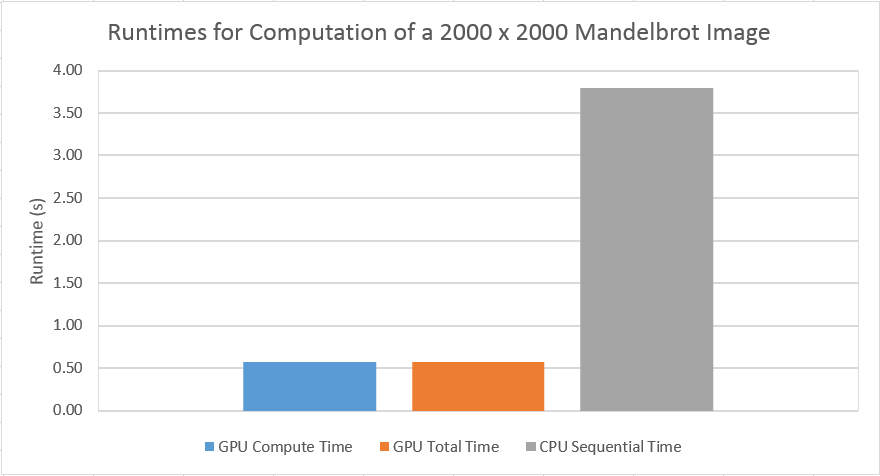
\includegraphics[width=.9\linewidth]{runtime}
  %   \caption{A comparison of the runtimes for computing a 2000x2000 Mandelbrot image using 1024 iterations at most for each pixel.}
  %   \label{fig:runtime}
  % \end{figure}

  % \begin{figure}[h!]
  %   \centering
  %   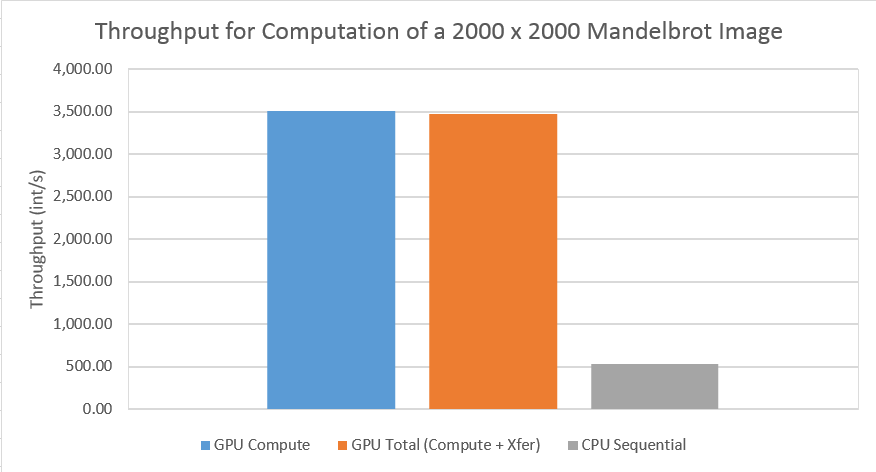
\includegraphics[width=.9\linewidth]{throughput}
  %   \caption{A comparison of the throughput in integer pixel values produced per second.}
  %   \label{fig:throughput}
  % \end{figure}

  % \begin{figure}[h!]
  %   \centering
  %   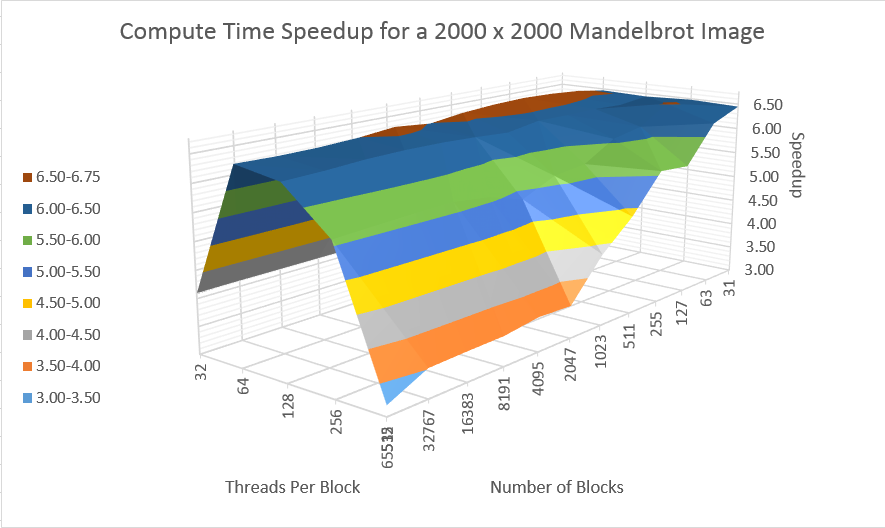
\includegraphics[width=.9\linewidth]{compute_speedup}
  %   \caption{The speedup achieved. Note the peak in the surface at 64 threads for all block sizes.}
  %   \label{fig:compute_speedup}
  % \end{figure}

  % \begin{figure}[h!]
  %   \centering
  %   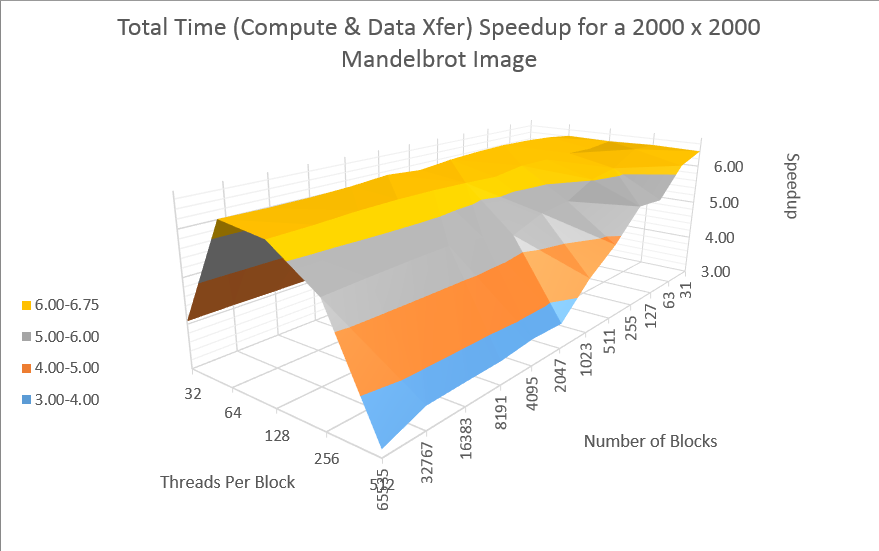
\includegraphics[width=.9\linewidth]{total_speedup}
  %   \caption{The speedup achieved when also considering the time to copy the computed data from the GPU to the Host.}
  %   \label{fig:total_speedup}
  % \end{figure}

  % \begin{figure}[h!]
  %   \centering
  %   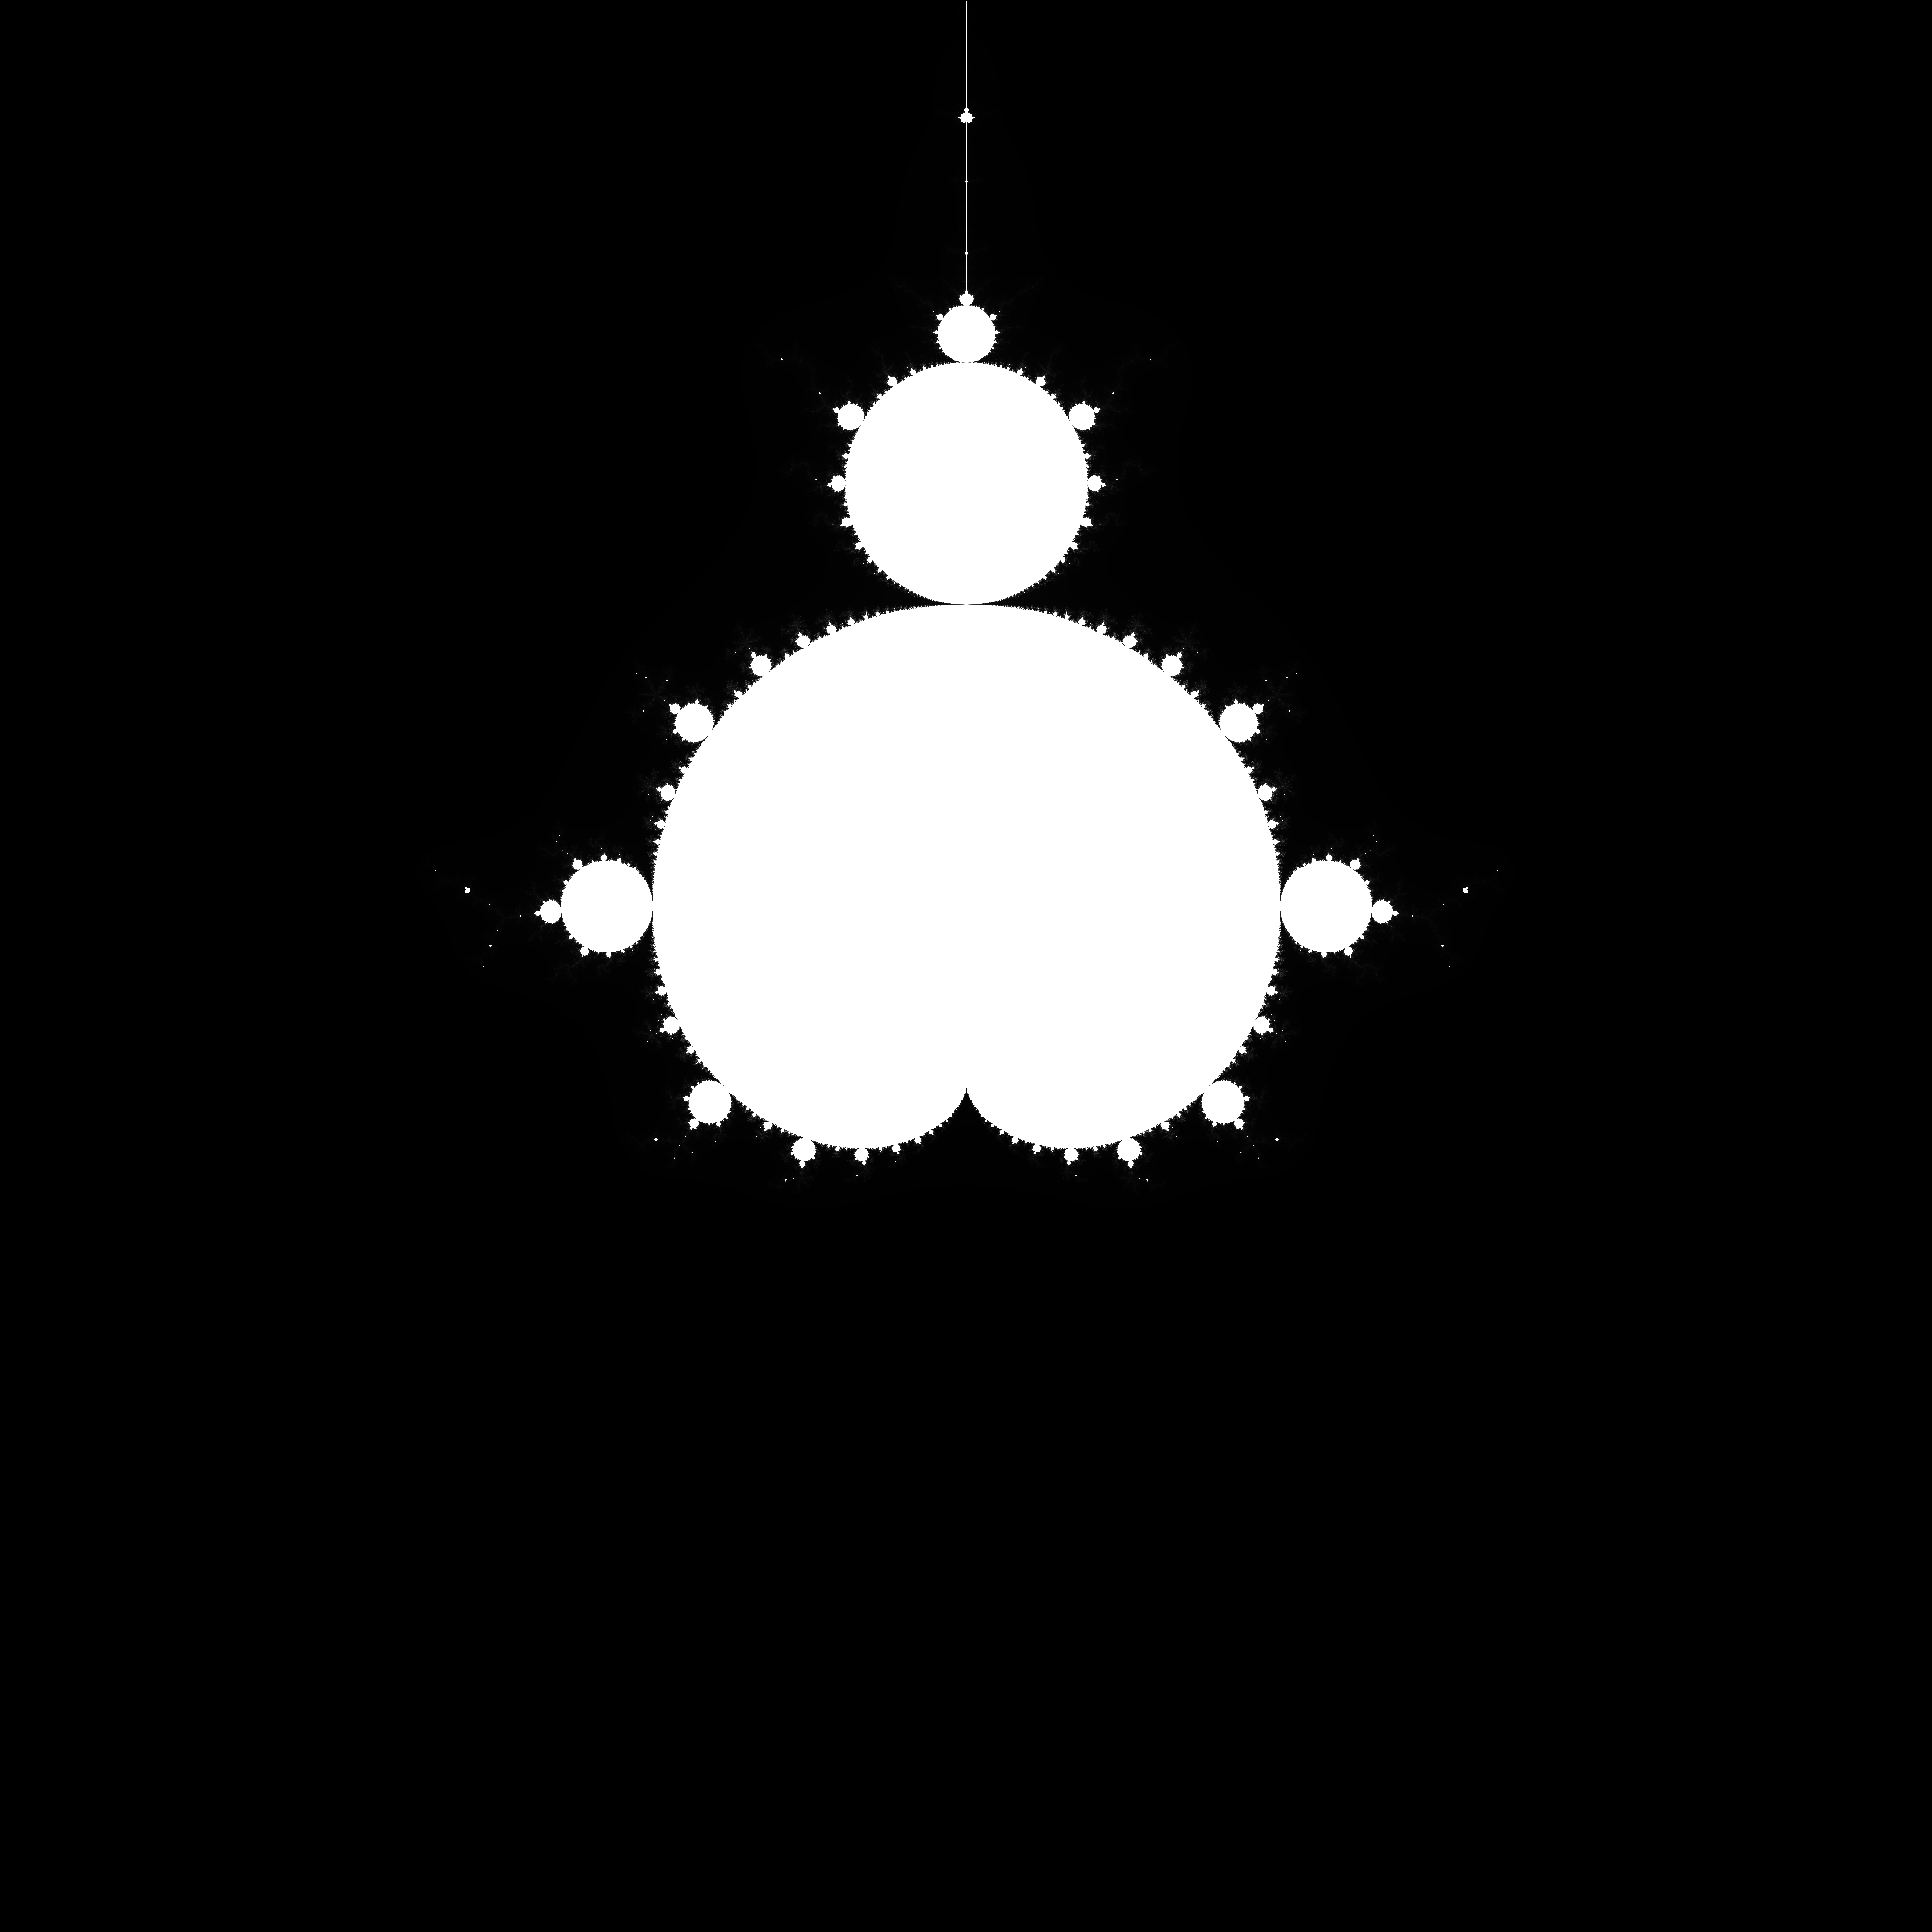
\includegraphics[width=.7\linewidth]{testimage}
  %   \caption{A Mandelbrot image for verification.}
  %   \label{fig:total_speedup}
  % \end{figure}

\newpage
\section{Discussion}


\section{Issues}

  
\end{document}
